\section{Résultats}

\paragraph{Étalonnage des transformateurs}
Les cycles à vide des transformateurs permettent de trouver \(\alpha\) tel que \(V_y = \alpha V_x\). Une régression linéaire sur le cycle du transformateur PHYWE à la \autoref{fig:phywe_vide} permet d'obtenir \(V_y = (truc) V_x\). Une régression linéaire sur le cycle du transformateur cylindrique à la \autoref{fig:cylindre_vide} donne \(V_y = (truc) V_x\). Le transformateur cylindrique ne présente pas d'hystérèse à vide, alors que le transformateur PHYWE possède une légère hystérèse, mais l'écart entre les courbes en montée et en descente est très faible, et les courbes restent linéaires sur une majeure partie du graphe.

\begin{figure}[h]
    \centering
    \begin{subfigure}{0.5\linewidth}
        \centering
        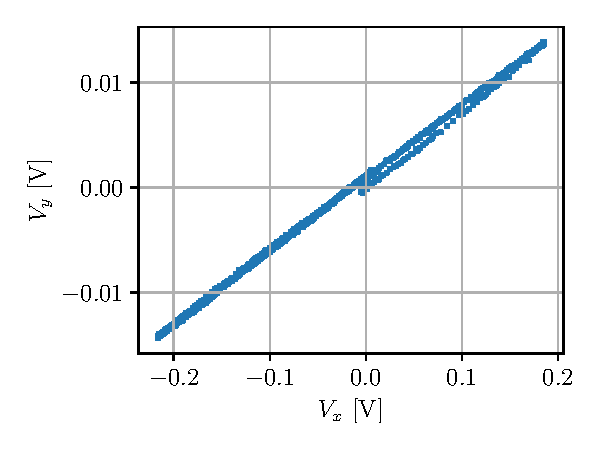
\includegraphics[width=\linewidth]{figures/G1-phywe-vide.pdf}
        \caption{}
        \label{fig:phywe_vide}
    \end{subfigure}%
    \begin{subfigure}{0.5\linewidth}
        \centering
        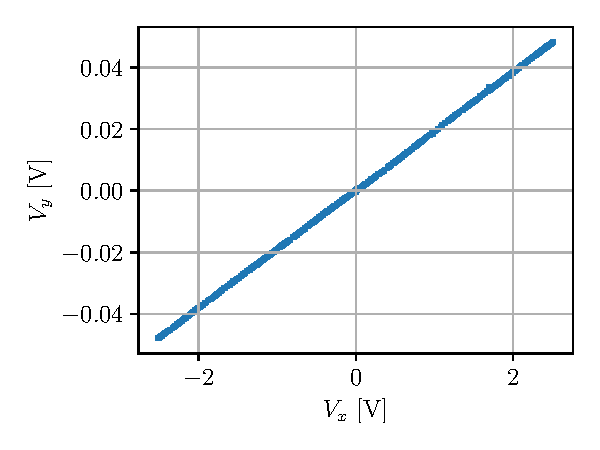
\includegraphics[width=\linewidth]{figures/G1-cylindre-vide.pdf}
        \caption{}
        \label{fig:cylindre_vide}
    \end{subfigure}
    \caption{Cycles à vide sur les transformateur (a) \textit{PhyWe} (b) cylindrique}
\end{figure}

\paragraph{Propriétés des matériaux}
MARTIN

\paragraph{Callibration des axes}
A VOIR @MARTIN

\paragraph{Trucs supplémentaires}
Titre à revoir, en gros les différents cycle d'hystérèse, les différentes épaisseurs, les plaques amagnétiques...

